\documentclass{UoYCSproject}
% Preamble
\usepackage{url}     % This is needed for IEEE referencing
\usepackage{bookmark}
\usepackage{algpseudocode} % Pseudocode algorithm
\usepackage{algorithm}
\usepackage[backend=biber]{biblatex}
\addbibresource{references.bib}
\usepackage{graphicx}
\graphicspath{ {./images/} }

% Title Page
\author{Babar Khan}
\title{Predicting Memorable Regions Of Images}
\date{2023-April-23}
\supervisor{Adrian Bors}
\SWE

% Document
\begin{document}
\pagenumbering{roman}
\maketitle

\tableofcontents

\chapter{Executive Summary}

%The purpose of the research (what's it about and why's that important)
I investigate a range of deep conditional image to image generative models and their success in learning mappings of images to memorable regions across three different experiments. If successful these models could be used by marketers, educators, or any creators to determine which parts of their images are memorable, and thus help to more easily create memorable images.
%The methodology (how you carried out the research)
This was done by conducting supervised training using image, VMS pairs in the VISCHEMA dataset. I compare these models using the L1 loss of their predicted memorability maps across the validation portion of the dataset.
%The key research findings (what answers you found)

I have found that autoencoders learn a somewhat accurate mapping but tend to smooth out the blocky VMS components into circular shapes, generally they took the least amount of time to train of the three models proposed, and achieved a mean L1 loss of \(\sim 0.132\) across the validation distribution. 
GAN models can be difficult to work with, and lots of research has gone into creating versatile and robust GAN architectures, adapting an existing, successful, model to your needs can reduce development time. Using a modified pix2pix GAN model \cite{isola2018imagetoimage} I was able to generate very accurate VMS maps, maintaining the blocky shape of the regions, and achieving a mean L1 loss of \(\sim 0.0740\). Generally, these models took longer to train than my autoencoder models.
% This is subject to change
Diffusion models took the longest to train, and while they can generally produce high quality images \cite{ramesh2022hierarchical, saharia2022photorealistic}, the training loop requires a large amount of computational resources, making it difficult to fine tune in a reasonable time. My best model was able to achieve an L1 loss of (Final Diffusion Loss). Due to computational restraints I was unable to run a large hyperparameter search and my results leave room for improvement.
% FILL IN FINAL DIFFUSION LOSS
%The implications of these findings (what these answers mean)

I show that using a GAN model we are able to predict memorable image regions with great accuracy.. I believe this has many useful applications across many different industries, allowing creators to have a more informed opinion on which sections of their images are memorable, using this tool to iteratively improve their image memorability. Hopefully in future work good parameters can be found that allow diffusion models to work with lower noise steps and to produce higher accuracy results.

\chapter{Reflections}

%my own experience 1/2 pages separate count?


%  learning to use Latex


%  working in the library vs training my models


%How difficult was to find resources for the project (data, computation)


% Identifies experienes that have had significance
% Can identify specific incidents and activities of significance to their learning
I found a great interest working on this project on as I'd never created an image to image model, considered the memorability of images, or even read a research paper before starting. Luckily my project supervisor, Adrian Bors, suggested a range of great research papers on image memorability, and that allowed me to start with a good footing.

There is a lot of openly available research into machine learning and computer vision, AlexNet \cite{alexnet} sparked somewhat of a machine learning renaissance in 2012, and in the decade since we have seen countless incredible papers released. The industry as a whole is very open, not only do academics produce research but large companies with huge funding typically post their research online for anyone to read. This abundance of research makes getting up to speed on the state of the art very easy. Not only is there a lot of free research available, but there are also countless articles and videos produced with the aim of making learning concepts easier. 

A big challenge for me was reading and understanding lots of these maths heavy research papers, I would often have to read a paper multiple times until I truly got what was happening, this was difficult and required perseverence but now I'm more comfortable with having to spend a long time figuring out what a paper is showing.

My dissertation is written using LaTeX, and bar a few small hiccups, it was very easy to learn to use as there are lots of online resources available. I typically write notes in markdown, which are very similar to TeX files and I imagine made the transition easier than going from a traditiomal WYSIWYG editor to LaTeX. I had never used LaTeX before but I have grown very fond of it. 

I find it difficult to work at home, and prefer to work in the University Library or any of the other various study spaces available. Unfortunately, my laptop is not computationally powerful enough to train most deep networks, my workflow became a cycle of writing code at the library and running it on my computer overnight. This work structure did take a while to get used to but it didn't pose much of a hassle in the end. I could have theoretically set up a Jupyter remote server to run on my computer at home, and connected to that from my laptop, but I was concerned about SSH vulnerabilities. If I were to do this proejct again I would spend the time learning how to set up a Jupyter server as I could have been far more productive. I considered training on Google Colab but unfortunately I hit the free GPU usage limit very quickly and decided that it is unreliable. 

% Makes a clear case for learning from an experience
% Identifies learning from an experience in a logical and credible fashion. Demonstrates links between the experience and the learning considering: elements of personal challenge: tangible evidence that the learning has taken place, ranges of learning from 'hard skills' through to personal insights

% Demonstrates the personal significance of the learning, including potential future value
% Understands and articulates the importance of the learning acquired. Potentially presents the role the learning might have in future activities; academic or professional

I would like to persue a career in computer vision and what I have learned working on this project will be immensely useful. My goal was to learn to predict memorability maps from images but while trying to achieve that I have learned so much in the surrounding areas of computer vision and deepened my knowledge of deep learning.

% Ability to honestly evaluate and critique personal performance in the context of the project
% Offers credible evaluations of personal performance relate to appropriate criteria. Evidence of mature consideratons of personal strengths and weaknesses. Consideration of the future implications of these insights



I've taken 3 courses at the University of York on inteligent systems, and in one of them implement my own unconditional GANs, because of that the transition to creating my own conditional image to image networks wasn't too foreign. One of my strengths is that I'm really able to stick to a problem for a long time, if something wasn't working I would happily spend hours fixing it without needing a break.  

Unfortunately diffusion models take a long time to train, and even longer to evaluate over the approximately 300 images in the VISCHEMA validation set, to evaluate one of my diffusion models with 2000 noise steps over the entire validation dataset would take roughly 4 hours, compared to the seconds for an autoencoder or GAN. This has meant that my third experiment took significantly longer to run than the first two, and has been the cause of many headaches. I regret that I was unable to achieve great results using a diffusion model and wish I had spent more time getting them to work, I spent too much time perfecting my Autoencoder and GAN results and should have spent more time on the diffusion, I naively assumed that it would take a similar amount of time to get good results with all three.

% Writes clearly and appropriately for the context of the report
% Writing is clear, concise, and clearly foxused around the evaluation of personal learning and performance on the project. Considers personal development alongisde technical skills aquired.

Overall I am proud of the work produced in this project, I have learned a lot about computer vision and memorability and I have produced, what I would consider, great results.

\chapter{Introduction}

% This should be 2 pages
% need to define well what i am doing

\section{Background}

%We see a lot of images

We are constantly surrounded by imagery, on the way to work, on the internet, on TV, in stores, just to name a few. Some images stick out more than others, we see hundreds, if not thousands, of images a day, and yet culturally and individually we all remember similar ones. 

Due to cultural significance an image can become memorable. The 2015 dress \cite{BBCDress2015}, a country's flag, or the 1932 image “lunch atop a skyscraper” \cite{gambino_2012}, come to mind. I argue that the memorability of such images is tied to the culture surrounding them, not necessarily due to intrinsic properties within. The focus of this research is on the intrinsic properties within an image that make it memorable to an individual, akin to seeing an advert on a bus and then later recognising the same advert online.

%How do we measure the memorability of an image

% What work has shown independence of memorability from viewer?
% Isola et al in 2011
% Vischema dataset experiments

It has been shown that the memorability of an image is an intrinsic property, independent from the viewer \cite{Isola2011, IsolaParikhTorralbaOliva2011, ICCV15_Khosla, isola2014memorability}, This is taken further by Akagunduz et al. \cite{VischemaPaper} where, in a similar experiment, they measure which regions of images are memorable.

\section{Motivation}

% Why do we want to do this

%Why do we want to create a memorable image
%How does this research help to create a memorable image

Creating memorable images is the goal of many industries, in education you want to create learning resources remembered by students, in marketing, adverts remembered by customers, and in movies, scenes remembered by audiences.  Its been shown that with great accuracy we can train a deep neural network to predict the memorability score of an image \cite{Isola2011, IsolaParikhTorralbaOliva2011, ICCV15_Khosla, isola2014memorability},
% Double check sources
that is, assign a float in the range of [0,1] to an image, with a higher score indicating higher memorability. But I propose that the memorability of an object within an image may be independent from the memorability of that object on its own. For example, an advert's memorability may not be equal to the memorability when seen in an environment such as on the side of a bus or building, in these cases the advert competes with everything else the viewer observes. This gives great importance to the examination of image region memorability, hypothetically a person wanting to create a memorable image could render their image on the side of a bus or building digitally, and test the memorable regions of that rendered image. They could then iteratively modify and examine their image until it is the most memorable region of the scene.

% What motivates me

%What are my goals

This is an incredibly difficult task, success has been found in semantic image segmentation \cite{wang2023internimage} and I believe that this task is a continuous variation of it. My motivation with this work is to both gain a deeper understanding of image memorability, and to gain experience using image to image deep convolutional networks. I want to create an accurate mapping from image to memorability maps. As I am using the VISCHEMA dataset in a supervised learning environment, I can measure the accuracy, or success, of my models as the L1 loss between my network output and the ground truth label present in the dataset. I would also qualitatively analyse the network outputs as the models may learn tricks that give a low L1 loss but don't look like the original labels.

\section{Report Structure}

The next chapter is my literature review, I cover prior research in image memorability and offer a brief overview of existing image to image models.

The following chapter is the methodology of my report, I describe three experiments where I test the ability of different models to predict the memorable regions of images when trained across the same dataset.

After that is the section on my experimental results, where I discuss in detail my findings across the three experiments.

Finally, the conclusion, where I discuss the implications of my findings.

\chapter{Literature Review}

% This should be 6-8 pages long

\section{Memorability}

% Roy Brener An experimental investigation of memory span
% Subjects were presented with units of varying length and were asked to recall them
% The unit could be a sentence, a digit, a geometric shape, etc
% It was found that people are not very good at remembering nonsense sylables or sentences but are much better at remembering digits, consonants, and colours. Remembering geometric designs is placed somewhere in the middle.
% This would seem to indicate that people are not very good at recalling images, however in Nickerson's work we can see that subjects are extremely good at recognising images. 

% R. Nickerson Short-term memory for complex meaningful visual configurations 1965
% Subjects are shown new and old photos and they have to identify if the photo is new or old
% P(Ro/So) = ~0.9
% 95% of all responses were correct
% subjects were more likely to correctly identify a photo as new than they were to correctly identify a photo as old
% Shown 1 image at a time with 50% chance of being old and 50% chance of being new
% 

% L. Standing. Learning 10,000 pictures. In Quarterly Journal of Experimental Psychology, 1973
% ## What is the goal of this paper ##
% Memory capacity and retrieval of pictures and words
% it shows that the capacity for memory of pictures is almost limitless, when measured under appropriate conditions. 
% People are able to recall images incredibly well  
% ## What are its limitations ##
% The experiments don't have many people involved Experment 2 only has 2 subjects and experiment 4, 4.
% He tested normal and vivid pictures
%------------

% F. Brady, T. Konkle, G. A. Alvarez, and A. Oliva. Visual long-term memory has a massive storage capacity for object details. In Proceedings of the National Academy of Sciences, 2008
% This is about how much detail is required to remember an image, rather than if you can just remember it or not
% Are you truly only able to store the gist of items in your long term memory, or are we capable of more?
% It is shown that people are able to store far more information than just the gist in their long term memory, we are able to store fine grained details
% this builds directly onto the world of Standing in 1973
%------------

In Breners work \cite{BrenerMemorySpan} subjects' abilities to remember a series of units was tested, with units defined based on the test performed, 
\begin{quote}
    In the digit test, for example, each digit was a unit; in the sentence test each sentence was a unit, etc. ... Each nonsense syllable constituted a unit ... Each consonant constituted a unit ... Each [geometric] design constituted a unit. \cite[p.468]{BrenerMemorySpan}
\end{quote}

It was found that people are not very good at remembering nonsense syllables or sentences but are much better at remembering digits, consonants, and colours. Remembering geometric designs is placed somewhere in the middle. This is of interest because it's very similar to our investigation into what aspects make images memorable. Brener was interested in consonants, colours, geometric designs, and other units, and his finding that different units can be significantly harder or easier to remember is useful to us. If we swap out units for image properties such as texture, contrast, saturation etc, or even more abstract features that a CNN may recognise, then it should be possible to find how memorability is impacted by these.   

The mean score of 5.31 found for geometric designs seems to indicate that people are not great at recalling images, however in Nickerson's work \cite{NickersonShortTermMemory} we can see the opposite, subjects are found to be extremely good at recognising images. Nickerson found that subjects shown a series of images are, with great accuracy, able to recall if the photo is one they have seen before or not. An item is referred to as 'new on its first occurrence and old on its second occurrence'\cite[p.156]{NickersonShortTermMemory}, it was found that subjects shown one image at a time, each with equal chance of being old or new, are able to correctly distinguish them with 95\% accuracy. 

Like in \cite{NickersonShortTermMemory}, Shephard's work \cite{ShepardRecognition} also found that subjects are able to distinguish with great accuracy new and old images, the mean percentage of images correctly identified was 99.7\% after a delay of 2 hours, 92.0\% after a delay of 3 days. 87.0\% after a delay of 7 days, and 57.7\% after a delay of 120 days. The introduction of a delay into Nickerson's experiment allows us to see that regardless of whether the image is in our short-term memory (2 hour delay) or our long-term memory (3-120 days) subjects are able to correctly identify an incredible amount of images. 

Standing built on the work of Nickerson, Shepard, and Brener in \cite{standing10000pictures}. Four experiments were ran which tested memory capacity and retrieval speed for pictures and words, I am interested in the performance related to pictures specifically. He found that, when measured under testing conditions, the capacity for image recognition from memory is almost limitless. In Standing's first experiment he tested 'normal' and 'vivid' images. He describes 'normal' images as those that 'may be characterized as resembling a highly variegated collection of competent snapshots'\cite[p.208]{standing10000pictures}, and 'vivid' images are described as 'striking pictures ... with definitely interesting subject matter'\cite[p.208]{standing10000pictures}. Much like how in Brener's work \cite{BrenerMemorySpan} the memorability of an object was variable based on what classification of unit was tested, this work shows that on an even more specific level, the classification of the image into normal or vivid, has an impact on subjects' memory, Standing found that the vivid images were more likely to be remembered by subjects.

Lots of work has been done to further build on that of Standing, Nickerson, Brener et al. Brady et al. \cite{brady2008visual} performed research into how much information is retained in long term memory and found that subjects are able to remember not just the gist of an image, but also fine grain information such as the state of objects within an image, and that they are able to distinguish between variants of objects shown in images. An example shown was an abacus in two different states, 13/14 subjects were able to distinguish which one they had seen before.

% D. A. Brown, I. Neath, and N. Chater. A temporal ratio model of memory. Psych. Review, 2007.
%An exploration to the extend to which common retrieval princples apply to human memory over short and long timescales
% Traces of items are represented in memory partyly in terms of how long ago they were observed
% Similar mechanisms govern retrieval from memory over many different timescales

Konkle et al. build further on the work in \cite{standing10000pictures, brady2008visual} by studying the impact that categorical distinctness has on memorability. This was tested by creating a dataset of images composed of categories such as tables, cameras, and bread etc. Each category had between 1 and 16 images, and a memory test like those performed in \cite{standing10000pictures, brady2008visual}
% check which other memory tests this matches
was performed. The percentage correctly identified was found to decrease as the number of images within a category increased, from this we can see that categorically distinct images are more likely to be remembered. 

Studies by Isola et al. \cite{Isola2011, IsolaParikhTorralbaOliva2011} were performed with the goal of identifying a collection of visual attributes that make images memorable, and to use those to predict the memorability of an image. It was found that properties such as mean saturation, and the log number of objects, has less impact on the memorability score than object statistics. 
%WTF are object statistics?
Categories such as: person, person sitting, and floor, were most helpful image memorability. The categories: ceilings, buildings, and mountains, were least helpful. Their approach was limited by the fact that the object statistics were annotated by hand, this would both make automating the process of determining image memorability impossible, and limit them from finding any abstract properties that helped/hindered memorability.

Khosla et al. \cite{NIPS12_Khosla} built on the work in \cite{Isola2011, IsolaParikhTorralbaOliva2011} by, instead of determining memorability of an entire image, creating a model that discovers memorability maps of individual images without human annotation. These memorability maps are able to distinguish which areas of an image are remembered, forgotten, or hallucinated. Their approach, similar to Isola et al. in \cite{Isola2011, IsolaParikhTorralbaOliva2011}, is limited by the arbitrarily picked list of features that define memorability.

\section{Using Deep Learning to Predict Memorability}

% How do I want this to flow?
%   Deep learning intro? talk about it being an image segmentation problem and something about convolution and learning filters
%   Possible Datasets
%   Auto Encoders (UNET)
%   GANS
%   Diffusion

\subsection{Memorability Datasets}

% Understanding and predicing image memorability at a large scale
%A novel experimental procedure to objectively measure human memory, allowing them to build LaMem, the largest annotated image memorability dataset
% How is it annotated? Memorability Scores in range [0,1]
% Heat maps?
% They show that fine-tuned deep features outperform all other features by a large margin
% They use Hybrid-CNN to classify the categories of objects and scenes. 

%What are deep learning models - 1 sentence
Deep learning models are composed of a large number of simple functions, these functions have adjustable weights that can be tuned to produce a more optimal output. A loss function is used to calculate how correct the output of the model is, and then each weight, W, is updated by calculating $\frac{\partial L}{\partial W}$ and performing gradient descent.
%There are two ways to train deep learning models, supervised and self supervised. The goal of supervised a learning is to learn a mapping between given input, label pairs. This requires a large pre annotated dataset to work off of. 

Deep learning models can be trained through supervised or self-supervised learning. In supervised learning the model is trained across a pair of input and output pairs, this requires a pre-annotated dataset to train on. This process can be costly and it's important to train on a dataset without any biases, as these can appear in your final models \cite{dastin_2018, najibi_2020}.  

% Talk about LaMem and how they created this dataset, its strengths and its weaknesses
% Talk about VISCHEMA and its strengths and weaknesses.
There are two datasets of interest. LaMem \cite{ICCV15_Khosla}, created by Khosla et al., and VISCHEMA \cite{VischemaPaper} created by Akagunduz et al. 

LaMem contains 60,000 annotated image and memorability pairs. Memorability is measured as a continuous value in the range [0,1] where a higher value indicates that the image is more memorable. They then train a CNN to predict the memorability of an image, resize their images, and pass overlapping regions of the image into their CNN. The generated memorability maps are tested for accuracy by adjusting the original images to de-emphasise the regions indicated as memorable. These adjusted images are then tested using the original memorability game used to create the dataset. They find that their memorability maps do reliably identify memorable regions.
% How is memorability scored.
% what is rank correlation
% Optimised protocol of the memory game introduced by [13] -> P. Isola, J. Xiao, D. Parikh, A. Torralba, and A. Oliva. What makes a photograph memorable? 

VISCHEMA is a significantly smaller dataset, containing around 1600 images, memorability map pairs in the VISCHEMA Plus version. Their experiment differs from that of Khosla et al., they ask participants to memorize a set of images, and then during a test phase rate how well they remember each image and to select the regions that made them remember it. In order to predict memorability the network output utilises fully connected layers which I believe is unnecessary, and may even hurt performance. More modern computer vision network structures, such as those in \cite{ronneberger2015unet, goodfellow2014generative, ho2020denoising, isola2018imagetoimage, saharia2022palette}, use fully convolutional networks. These maintain spatial locality which allows them to generalise better.


\subsection{Image Synthesis Models}

\subsubsection{Autoencoders}

The autoencoder model is composed of 3 parts, an encoder, a bottleneck, and a decoder, these are typically used for compression. The U-Net \cite{ronneberger2015unet} is a variation of an autoencoder which has found great success in semantic image segmentation within the medical field. It makes use of residual connections between corresponding layers in the encoder and decoder blocks, these allow the model to preserve data for use in the decoding stage. This architecture is the backbone of many image to image models \cite{isola2018imagetoimage,saharia2022palette,dhariwal2021diffusion}, and has seen many extensions \cite{zhou2020unet, Qin_2020}

\subsubsection{Generative Adversarial Networks}
% in 2018? ns on the date, pix2pix was invented, it is a GAN built around the UNet and has also seen great success

% need to introduce GANs, their weaknesses and their benefits

% You typically cant track the progress of a GAN by looking at the loss of the generator or the discriminator, however after running an epoch of training I can compute the loss of the generator across the validation dataset, independent of the discriminator, this allows us to track the progress of the generator and compare it to other methods.


% Maybe here say what a GAN vs a conditional GAN is 

GAN architectures\cite{goodfellow2014generative} use competitive co-evolutionary algorithms where a Generator and a Discriminator compete. The Generator is typically given a latent space vector and uses that to produce an image, the Discriminator has to determine if that image belongs to a given distribution. Conditional GAN architectures use an encoder to transform an image into a latent space vector and then a decoder to transform that back into an iamge, these networks have seen great success \cite{zhu2020unpaired, karras2019stylebased, isola2018imagetoimage} but are typically unstable and require a lot of parameter fine tuning. They can also suffer from: non-convergence, mode collapse, and diminished gradients \cite{goodfellow2017nips}.

\subsubsection{Diffusion Models}

% talk about significance of diffusion, its benefits and weaknesses
% how it builds ontop of GANs and why they have seen so much success recently

Diffusion based generative models work by learning to iteratively remove Gaussian noise from a sample T times until it produces an image from the training domain. The model was first proposed by Sohl-Dickstein et al. \cite{sohldickstein2015deep}, and has been further developed by Ho et al. \cite{ho2020denoising},  Dhariwal and Nichol \cite{dhariwal2021diffusion}, and Saharia et al. \cite{saharia2022palette}. They are a machine learning model that work through a forward diffusion process systematically destroying the structure in a data distribution, and the learning of a backwards process to restore the structure. The method uses a Markov chain to convert $ x_t $ into $ x_{t-1} $. Starting with $ x_T $, a sample of Gaussian noise, a generative Markov chain converts this into $ x_0 $, which is a sample from the target data distribution. Because the model only estimates small pertubations of noise, $ x_t $ given $ x_{t-1} $ , rather than an entire transformation from $ x_0 $ to $ x_T $, it is tractable to train. 

The DDPM is a diffusion model capable of producing high quality images and achieves state of the art FID scores across the CIFAR10 dataset \cite{ho2020denoising}. Dhariwal and Nichol \cite{dhariwal2021diffusion} show tweaks that allow for diffusion models to achieve state of the art FID scores across the ImageNet dataset and when used in combination with upsampling diffusion further improve FID scores. They do this by using improvements proposed in \cite{song2022denoising, nichol2021improved, song2021scorebased, brock2019large, karras2019stylebased}. 

%These improvements also reduce the number of noise steps required from thousands to (in some cases) 50. Through the decrease in noise steps they are able to reduce the amount of time that it takes to generate an image. Chen discusses in \cite{chen2023importance} how changing the resolution of an image has an impact on the noise scheduling required, he finds that the optimal scheduler at a smaller resolution may cause under training for higher resolution images. Multiple strategies are proposed to adjust noise scheduling. Firstly, changing the noise schedule functions to those based on cosine or sigmoid, with temperature scaling. Secondly, reducing the input scaling factor from 1 increases the noise levels which destroys more information at the same noise level. They then combine these into a compound noise scheduling strategy.


\chapter{Methodology}

% I dont think this needs to be long, ~2 pages
% This should be from a theoretical perspective
% No need for specific values, just describe what I plan on doing
% Use general ranges of the params

% Motivation?

\section{Requirements Capture}

The two dataset options I have considered are LaMem \cite{ICCV15_Khosla} and VISCHEMA \cite{VischemaPaper}. I have chosen to use the latter to train my image to image network because Akagunduz et al. successfully measure the memorable regions of images, rather than a score per image, while Khosla et al. are able to convert these scores into memorability maps, that is inherently less robust than the experiment presented in \cite{VischemaPaper}. I'm also not convinced that the memorability of an image stays the same if that image is part of another image, for example if a person saw an image of an advert vs an image of that same advert on the side of a bus, it doesn't seem intuitive to me that the advert would be just as memorable in both cases.   

The VISCHEMA Plus dataset contains 1600 image to VMS mappings, 1280 of these compose the training portion and the remaining 320 the validation portion. I aim to use a range of deep convolutional image to image model to learn a mapping of these images to their corresponding VMS labels. Our models should learn a general understanding of the mapping such that when it is provided with an image that matches our distribution, it can accurately create a VMS label for it. Our model will be successful if they can learn to create accurate mappings across the validation dataset, I will evaluate accuracy using the L1 loss function and through qualitative analysis. 

\section{Ethical Concerns}

I have adapted and used code available in the following repositories \cite{PytorchPix2Pix, JanspiryPalette}, both have licenses that allow their use in this project. I have also used the VISCHEMA dataset \cite{VischemaPaper} to train my models. All other contributions have been referenced. 

\section{Motivation}

As autoencoders, GANs, and diffusion models all produce images in different ways. Autoencoders learn to produce output images directly through the backpropagation of the loss between its output and the ideal output. GAN generators learn to produce images by tricking a discriminator. Diffusion models learn to produce images by removing noise from latent space iteratively. I think it would be interesting to compare how the 3 of them perform when asked the same task. I will run three experiments where I train a UNet autoencoder, a GAN, and a diffusion model to produce a VMS label given an image from the dataset. I hope to be able to find the strengths and weaknesses of each of these systems in this application. For each model I will experiment with network parameters and training hyperparameters to fine tune models that produce the best output.


In each experiment I will automate a system that: tests the effectiveness of different numbers of layers and channels in each network, varies the normalisation method, optimisation function, learning rate, and batch size to find the best training environment and model parameters. It is not be feesible to test every combination of these variables, thus I will employ a training strategy to test every variation of a single parameter/hyperparameter while keeping the rest constant.


I will start each model with an estimation of good parameters, then iterate through each individual parameter, varying only that one and measuring the impact on performance. After testing all variations of a single parameter, I will pick the one that gave the highest score and move onto the next parameter. This will bring the size our search space down by an order of magnitude, however we won't be exploring the entire search space and will potentially miss out on good models. 


This training strategy will be especially necessary in experiment 2 as training within a GAN is typically unstable and good parameter choices are necessary. In experiment 3 I will also vary the noise scheduler and the beta values.

\section{Experiment 1}

The UNet is an autoencoder model presented in \cite{ronneberger2015unet}. Its original creation was for the purpose of image segmentation, because of this I think it should perform well in the task of generating VMS maps.

\textbf{Model}: I will use a UNet autoencoder that takes as input the images in our dataset.
% double check this input range
It outputs a 64x64x3 tensor of floating point values in the range [-1,1], these are our label estimates.
% double check this output range
This model can be described as: \[ L_{pred} = model(I) \]

\textbf{Model Loss}: This is simply the L1 loss between $L_{pred}$ and $L_{real}$, describing how closely the output of our network matches the corresponding label. At each epoch we will calculate this over the training dataset, update the model weights using the backpropagation of that loss, and then calculate the loss across the validaton dataset to test how well we have generalised.
\[ L = L1( model(I), L_{real} ) \]

\textbf{Training Strategy}: Please see algorithm \ref{ALG:Autoencoder} for the training loop.

\begin{algorithm}
\caption{UNet Autoencoder Training Strategy}\label{ALG:Autoencoder}
\begin{algorithmic}[1]
\For{$\texttt{every epoch}$}
\For{$I, L_{real} \texttt{ in training dataloader}$}
\State
\State $L_{pred} = model(I)$
\State $loss = L1( L_{pred}, L_{real} ) $
\State $\texttt{Update weights of model with backpropagation}$
\State
\EndFor
\EndFor
\end{algorithmic}
\end{algorithm}

\section{Experiment 2}

I will train a conditional generative adversarial network to generate images of VMS maps given images from the VISCHEMA dataset. I will use an adapted pix2pix network \cite{isola2018imagetoimage}, making tweaks that I think will increase performance. 
pix2pix by Isola et al.\cite{isola2018imagetoimage}, is an image-to-image conditional generative adversarial model based on the UNet \cite{ronneberger2015unet}. Designed to translate images from one style into another. In \cite{arjovsky2017wasserstein} Arjovsky et al. introduce a GAN variant based on the Wasserstein distance between the output distribution and the image distribution, the benefit of this is that the Wasserstein distance is continuous and differentiable almost everywhere, reducing the risk of dimminishing gradients. In \cite{pix2pixwasserstein} Makow investigated the use of Wasserstein Distance in the pix2pix model but unfortunately found that it does not perform much better, I would still like to experiment with it as VISCHEMA plus is different from any dataset used in \cite{isola2018imagetoimage} and as Makow states they were unable to perform a complete hyperparameter search, meaning that its possible we could achieve greater results than vanilla pix2pix.
I will be adapting the following Pytorch implementation \cite{PytorchPix2Pix} for my experiment. 

Lots of work has gone into making GAN models more stable and I will use these findings in my own models. In \cite{brock2019large} Brock et al. found that when 'increasing the batch size by a factor of 8 ... models reach better final performance in fewer iterations, but become unstable and undergo complete training collapse'. Because of this I will experiment with early stopping and low batch sizes.  In \cite{zhao2020differentiable} Shengyu et al. show how using differentiable augmentation on your images increases the quality of the outputted images. With a dataset with as few as 100 images they are able to produce high quality outputs, this is useful to us because the VISCHEMA plus dataset only has 1280 training images, which typically wouldn't train very well on a GAN.

% https://www.youtube.com/watch?v=J97EM3Clyys
% https://github.com/mit-han-lab/data-efficient-gans/blob/master/DiffAugment-stylegan2-pytorch/DiffAugment_pytorch.py
% horizontal flips are a good application on the real images
% You could augment the real images -> this will cause the generator to learn to generate augments, this is bad for augments such as cutout
% You could augment the real images and the fake images when the discriminator sees them, the generator will have an easier time fooling the discriminator
% Solution: Augment real and fake images for the discriminator and the generator
% Need to be able to differentiate the augmentation so that we can update the generators weights using gradient descent
% How do we make our augmentations differentiable?
% We provide a torch tensor that represents the images as input, then we randomly sample parameters related to augmentation. e.g. translation amount or cutout coords. Apply this augmentation to the input tensor
% since it is all done using torch operations, the computational graph will be computed for these functions
% Kornia can do this for us.
% pass the augmentation module, kornia, into the discriminator. Apply augments on the input to the discriminator first but only when training 

%https://cs230.stanford.edu/projects_spring_2018/reports/8289943.pdf 


\textbf{Generator}: This network takes as input a an image from out dataet and outputs its prediction of the corresponding label, it can be described as: \[ L_{f} = G(I) \]

\textbf{Discriminator}: This network takes as input the concatenation of an image from our dataset and either its corresponding label or a generated label. It outputs a 4x4x1 tensor of boolean values, where each value in this output represents whether it predicts if a 16x16x6 region of the input is real or generated.

The loss for each network is computed as described in \cite{isola2018imagetoimage}, across an entire batch of images and then the weights are adjusted with backpropagation. The optimiser used is one of the hyperparameters that we will search for.

\textbf{Generator Loss}: The generator loss describes how well it can trick the discriminator, and how closely its output matches the real label for the given image.
\[ L = MSE( D(L_{f}, I), 1 ) + L1(L_{f}, L_{r}) \]

\textbf{Discriminator Loss}: The discriminator loss describes how accurately it is able to predict, given a label and an image, if the label is real or not.
\[ L = 0.5 \times  ( MSE( D( L_{f}, I ), 0) + MSE( D( L_{r}, I ), 1) ) \]

Because these two loss values are relative to the performance of eachother they can't be used to see if our generator has converged on a solution. Therefore it is necessary, at each epoch, to also compute the L1 loss of the fake labels and real labels across the training and the validation dataset, as these values are calculated independently of the discriminator. This will inform allow us to see if the generator is overfitting, underfitting, or training well. 

\textbf{Training Strategy}: Please see algorithm \ref{ALG:GAN} for the training loop.

\begin{algorithm}
\caption{GAN Training Strategy}\label{ALG:GAN}
\begin{algorithmic}[1]
\For{$\texttt{every epoch}$}
\For{$I, L_{r} \texttt{ in training dataloader}$}
\State
\State $L_{f} = G(I)$
\State
\State $pred_{fake} = D(L_{f}, I) $
\State $loss_G = MSE( pred_{fake}, 1 ) + L1(L_{f}, L_{r}) $
\State $\texttt{Update weights of G with backpropagation}$
\State
\State $pred_{real} = D(L_{r}, I)$
\State $loss_D = 0.5 \times  ( MSE( pred_{fake}, 0) + MSE( pred_{real}, 1) ) $
\State $\texttt{Update weights of D with backpropagation}$
\State
\EndFor
\EndFor
\end{algorithmic}
\end{algorithm}

\section{Experiment 3}

I will adapt a PyTorch implementation of Palette \cite{JanspiryPalette} and train it to predict labels from the VISCHEMA dataset. Palette is a versitile conditional image to image diffusion model proposed by Saharia et al. \cite{saharia2022palette} that is able to uncrop, inpaint, colorize, and remove JPEG artifacts from images. Because of this versitility I think it could learn to predict VMS maps from images. The conditional image passed to the model will be the image from the dataset and the ground truth will be the label. This network takes as input the concatenation of an image and the noise added to the ground truth label after $t$ steps. It outputs an estimate of the noise added to the ground truth label at time $t-1$.
This model can be described as \[ noise_{pred} = model(I, t) \]

\textbf{Model Loss}: This describes how well the model can estimate the noise added to an image between time steps $t-1$ and $t$, it is computed across an entire batch of images and then the model weights are adjusted with backpropagation.

\[ L = MSE( model(I, t), noise_{real} ) \]

The loss calculated for backpropagation is relative to the performance in estimating noise added, not for the performance when calculating VMS labels. Because of this I will also have to calculate the L1 loss of the generated labels against the real labels. This will take a lot of computational time so I will do it at the end of training. I will be able to see if our model has converged by observing the backpropagation loss. 

\textbf{Training Strategy}: Please see algorithm \ref{ALG:Diffusion} for the training loop.

% Maybe theres a better way to write this?
% Look at the papers and see if its there
\begin{algorithm}
\caption{Diffusion Model Training Strategy}\label{ALG:Diffusion}
\begin{algorithmic}[1]
\For{$\texttt{every epoch}$}
\For{$I, L \texttt{ in training dataloader}$}
\State
\State $t = random(0, noise\_steps)$
\State $noise_{real}, L_{noisy} = noise\_image(L, t)$ \Comment{Apply t steps of noise}
\State
\State $input = concatenation(I, L_{noisy})$
\State $noise_{pred} = model(input, t)$
\State $loss = MSE( noise_{pred}, Noise_{real} )$
\State $\texttt{Update weights of model with backpropagation}$
\EndFor
\EndFor
\end{algorithmic}
\end{algorithm}

\section{Results Analysis/Testing}

After performing all 3 experiments I will compare the results across the validation dataset qualitatively and using the L1 loss. The L1 loss will tell me how statistically close the outputs are but through qualitative analysis I can see if the outputs actually resemble the true labels, or if the models have achieved a low L1 loss through some exploit. 


I can also compare the L1 loss across the training and validation sets to see if a model has generalised well, if the loss across the training dataset is much smaller/larger than the validation dataset then it will imply that the model has become overfit/underfit respectively. Ideally they should be similar. 


\chapter{Experimental Results}

% Approx 10-15 pages

% add plots and tables of results and explain them
% important facts in text
% compare loss functions
% explain dataset limitations
%    solved with gan
%    in experiments?

\section{Experimental Environment}

I have implement the experiments in Python using the PyTorch machine learning framework, however the methodology that I describe should produce the same results in any programming language or framework.

This model was trained on a computer using an RTX 3070 with 8GB of VRAM and an AMD Ryzen 3600 with 32GB of system RAM.
Testing the hyperparameter options for experiment 1 took approximately X days and I trained the final model over the course of 40 minutes.
% FILL IN X AND Y
Testing the hyperparameter options for experiment 2 took approximately 3 days and I trained my final model over the course of 5 hours.
% Need to double check that  
Testing the hyperparameter options for experiment 1 took approximately X days and I trained the final model over the course of Y hours
% FILL IN X AND Y

All experiments were performed with differentiable augmentation as described in \cite{zhao2020differentiable}. I performed translation and cutout, each with a 90\% chance.
% THAT PERCENT MAY CHANGE

\section{Hyperparameter tuning}

For experiments 1 and 2 I automated the process of exploring the parameter and hyperparameter search space. In my search I varied the following parameters: The normalisation layer used, the channel layouts used, the optimiser used, the learning rates for the optimiser, and, if the Adam optimiser was used, the beta values. Because training a diffusion model is far more computationally expensive than training an Autoencoder or a GAN I was unable to automate the process of tuning the hyperparameters in experiment 3. Training a GAN model on the VISCHEMA dataset would typically take around 100 minutes, but training a diffusion model would take around 20 hours due to the greater number of epochs required.


In experiment 2 I allowed for the generator and discriminator models to use different normalisation functions, optimisers, and learning rates. 


Exploring this search space exhaustively is unfortunately not feesible, there are over 5000 different combinations possible, and if I tested each combination once for 100 epochs then it would take approximately 300 days to test per experiment.
% double check these numbers
% should I describe this in my methodology or above?
% how long does it take to train an epoch?
Instead I will have to explore a subset of this search space. For each experiment I estimated some good default parameter and hyperparameter values, by varying these values I can lower the scope of the search space to 
% maybe I should get an exact value here instead of 100
approximately 100 combinations, which took \(\sim\)3 days per experiment to test. Unfortunately this does mean that not every combination has been tested, however we should achieve a good approximation of the best parameters and hyperparameters.


% Should this go at the end?
In experiment 3 I was only able to explore a small range of possible hyperaparameters and as such my results do not emulate the recent success found in diffusion based image generation.
% papers on the success of diffusion.
However, with a greater number of computing resources it may be possible to do so.

\section{Experiment 1}

In this experiment I trained a UNet to predict the VMS maps of images, I trained the model using backpropagation of the L1 loss of the model output given an image, and the corresponding label. 


Diagram of my model:

The best parameters and hyperparameters that I found for my model were the following:
% Input best hyperparameters

\begin{figure}[h]
    \centering
    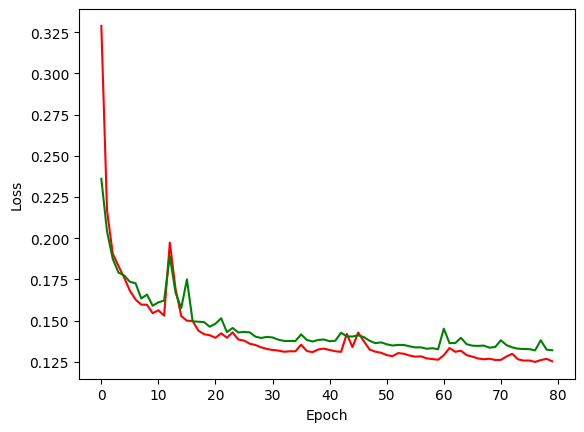
\includegraphics[width=\linewidth]{Autoencoder Training Curve}
    \caption{Autoencoder training graph. The red plot describes the training loss per epoch and the green plot the validation loss. The validation loss closely matches the training loss and the model does not become overfit.}
    \label{fig:autoencoderTraining}
\end{figure}


After 80 training epochs I was able to achieve an L1 loss across my validation dataset of ~0.132.

A sample of best output images:

\begin{figure}[h]
    \centering
    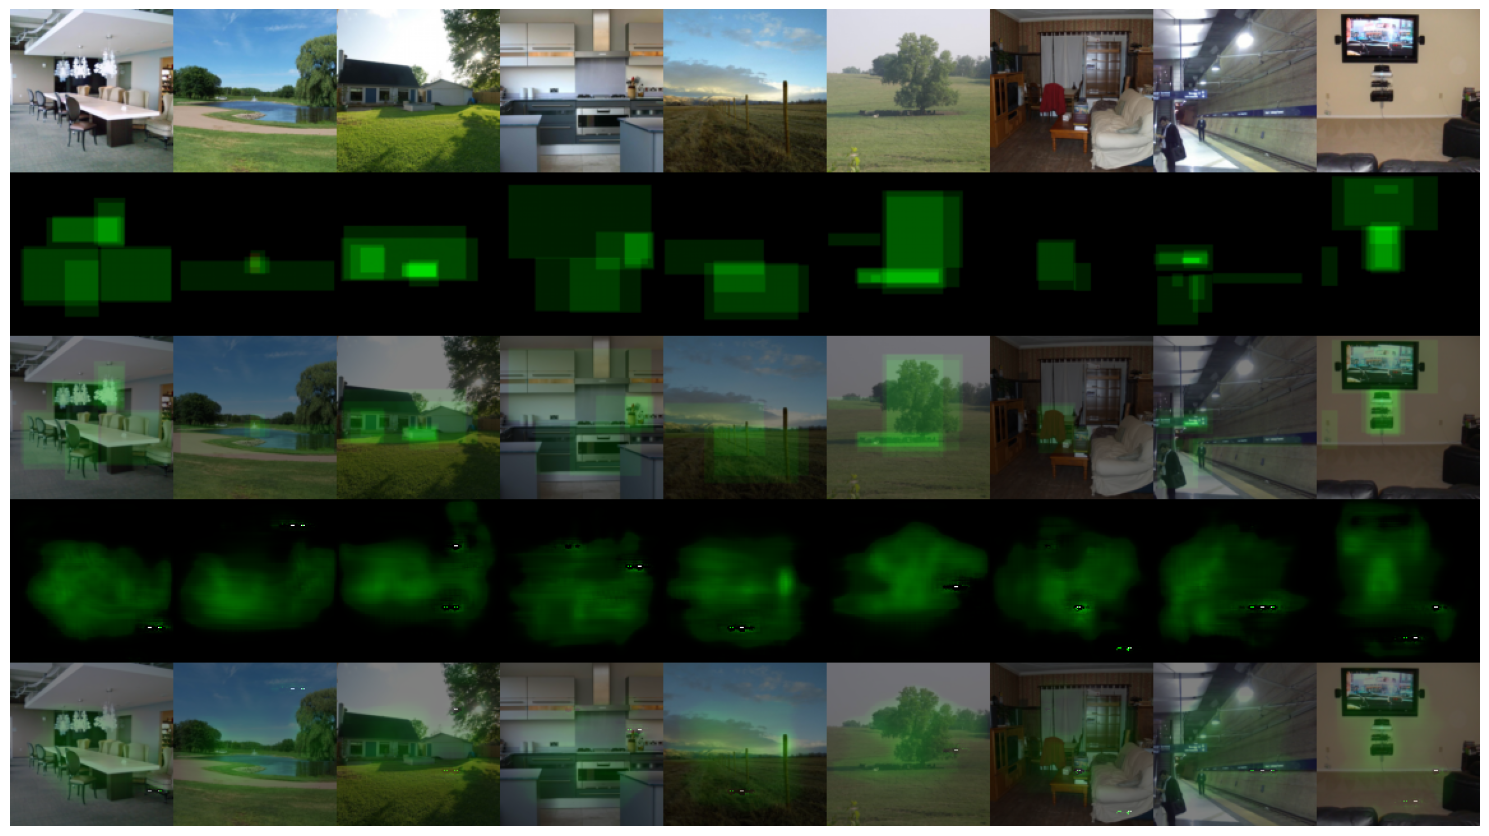
\includegraphics[width=\linewidth]{Best autoencoder Outputs}
    \caption{Best Autoencoder Outputs}
    \label{fig:autoencoderBestOutput}
\end{figure}

A sample of the worst output images:

\begin{figure}[h]
    \centering
    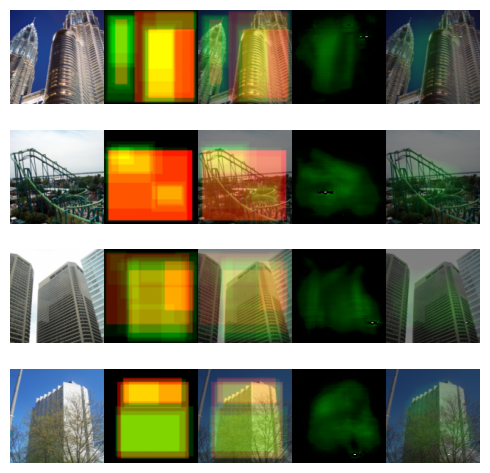
\includegraphics[width=\linewidth]{Worst autoencoder Outputs}
    \caption{Worst Autoencoder Outputs}
    \label{fig:autoencoderWorstOutput}
\end{figure}

When performed without differentiable augmentation the results looked like this:
% Images.

FID score of Z, L1 Loss of Y.
% Input Z, Y

\section{Experiment 2}

I explored the following parameter and hyperparameter options:

\textbf{Normalisation layers}: Batch Normalisation, Instance Norm

\textbf{Channel layouts}:
I iterated over generator encoder and decoder, and discriminator channel layouts of following form, with values of $c$ from \{32,64,50,100\}:
\begin{itemize}
\item Encoder: (3, $c$, 2$c$, 4$c$, 8$c$, 16$c$), 
\item Decoder: (16$c$, 8$c$, 4$c$, 2$c$, $c$),
\item Discriminator: (6, $c$, 2$c$, 4$c$, 8$c$, 16$c$).
\end{itemize}

\textbf{Optimisers}:
\begin{itemize}
\item SGD, using the following learning rates: 0.005, 0.01, 0.02,
\item Adam, using the following learning rates: 0.0005, 0.001, 0.002, and using the following betas values: (0.9, 0.999), (0, 0.999), (0.5, 0.999),
\item Adadelta, using the following learning rates: 0.5, 1, 2.
\end{itemize}

\emph{Note: I didn't need to specify default values for the normalisation layer as these were the first variables I tested.}

\textbf{Default Generator Parameters and Hyperparameters}: 
\begin{itemize}
\item $C$ = 64
\item Optimiser: Adam, betas = (0.9, 0.999)
\item Learning Rate: 0.001
\end{itemize}
\textbf{Default Discriminator Parameters and Hyperparameters}:
\begin{itemize}
\item $C$ = 64
\item Optimiser: Adam, betas = (0.9, 0.999)
\item Learning Rate: 0.001
\end{itemize}
I iterated over each different parameter and hyperparameter and varied each one sequentially. I tested each combination for 100 epochs and used the L1 loss across the validation dataset as the score, if any new parameter options gave a better L1 score the it would become the default used going forward. This meant that I only had to iterate \(\sim\)100 combinations. I found the following best options.

\textbf{Best Generator}: Batch Normalisation, $C$ = 32, SGD Optimiser with a learning rate of 0.01.

\textbf{Best Discriminator}: Batch Normalisation, $c$ = 100, Adam optimiser with betas = (0.9, 0.999) and a learning rate of 0.001.

With this combination we achieved a loss of \(\sim\)1.02 across the validation dataset. I found other good results using similar combinations. Using the Adatelta optimiser for the generator and the Adam optimiser for the discriminator achieved a loss of \(\sim\)1.03 across the validation dataset. Using the Adam optimiser for both the generator and discriminator achieved a loss of \(\sim\)1.04 across the validation dataset.

% THE ABOVE IS BS AND NEEDS CHANGING

After 200 epochs of training our model is able to achieve an L1 score of ~0.0740 across our validation dataset and Z across our training dataset.
% INPUT X, Y, Z
This is significantly better than our autoencoder model. 

Figure \ref{fig:GANBestOutput} shows the outputs across the validation portion of our dataset with the lowest L1 Loss. They're accurately labelled with the correct regions as memorable. 
but frankly are quite boring, the low L1 loss across these is because the labels simply have lots of black data, the loss across these is 0 if the model also outputs black. 
Figure \ref{fig:GANGoodOutput} shows what I think are far more impressive results, even if they have a higher loss than those present in figure \ref{fig:GANBestOutput}. For these images the model is able to accurately predict large regions of the image that are memorable.
The worst results are shown in \ref{fig:GANWorstOutput}, it appears that like our autoencoder model from experiment 1 that this model finds it difficult to predict regions that are detrimental to memorability. 

After 200 epochs, L1 Score of ~0.0740
% Insert X,Y

Here are the images generated when I dont use differentiable augmentation
% Insert images
% Insert training graphs

After X epochs L1 Score of Y
% Input X, Y

\textbf{Wasserstein GAN}: Using a Wasserstein image-to-image GAN as described in \cite{pix2pixwasserstein} I was able to achieve a best score of
% Insert score here.
% Insert images.

FID score of Z, L1 Score of Y
% Input Z, Y

Here are the images generated when I dont use differentiable augmentation
% Insert images
% Insert training graphs

FID score of Z, L1 Score of Y
% Input Z, Y

\section{Experiment 3}



\section{Results, Evaluation Metrics, and Analysis}

a graph of the train/val loss over time across the different experiments


a graph of the FID score at the end of the different experiments


a selection of the images with the different training methods


Some discussion about them.


\chapter{Conclusion}



% Approx 1-2 pages
% how it went
% future work better generator better result
% applications

% Put this in the conclusion
Diffusion models lend themselves well to multiple GPU architectures, and if I were to run this experiment again I would hope to have access to a system capable of running them faster. While diffusion models have seen lots of mainstream attention recently, until home computing power is significantly greater it is infeesible for most to train their own in any reasonable amount of time. 

Greater time means greater costs and until the hardware to run diffusion models increases in performance I can't see any benefits over using a GAN model.

Unfortunately I can't recommend the use of diffusion models to generate memorability maps, even if my models were able to generate accurate results, the time required using current hardware is simply too great.

\printbibliography

\chapter{Appendix}

Best results:
\begin{figure}[ht]
    \centering
    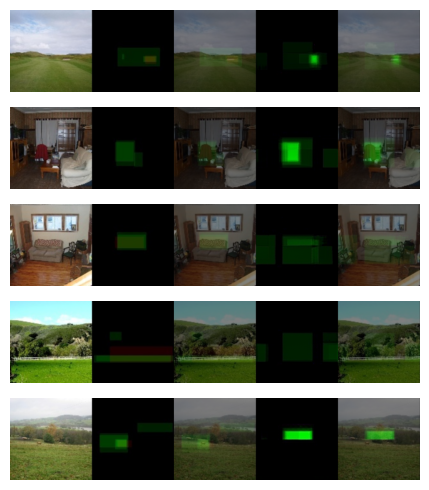
\includegraphics[width=\linewidth]{Best GAN Outputs}
    \caption{Best GAN Outputs}
    \label{fig:GANBestOutput}
\end{figure}

Favourite Results:
\begin{figure}[ht]
    \centering
    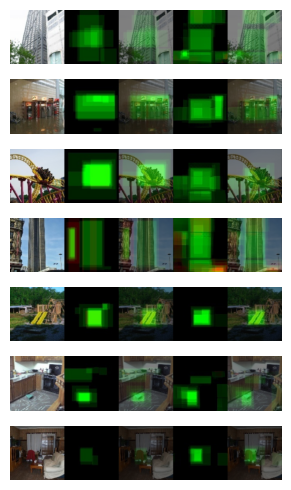
\includegraphics[]{Good GAN Outputs}
    \caption{Favourite GAN Outputs}
    \label{fig:GANGoodOutput}
\end{figure}

Worst results:
\begin{figure}[ht]
    \centering
    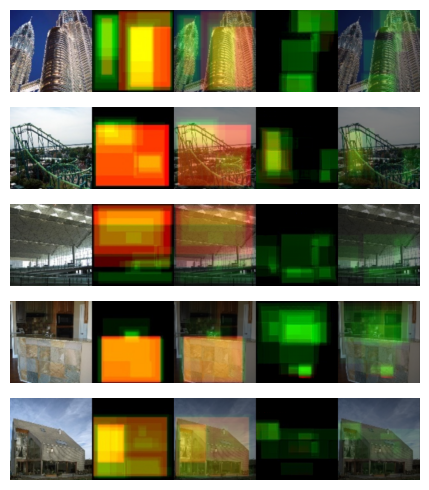
\includegraphics[width=\linewidth]{Worst GAN Outputs}
    \caption{Worst GAN Outputs}
    \label{fig:GANWorstOutput}
\end{figure}

\end{document}